\documentclass{beamer}
\usepackage{subfig}
\usepackage{amsmath}
\usepackage{bm}

\DeclareMathOperator*{\argmax}{arg\,max}
\DeclareMathOperator*{\argmin}{arg\,min}


\title{Model Selection and Bias-Variance tradeoff}
\author{Prof. Alessandro Lucantonio}
\institute{Aarhus University - Department of Mechanical and Production Engineering}
\date{?/?/2023}

\begin{document}
	\frame{\titlepage}
	
	\begin{frame}
		\frametitle{Motivations - Training vs test error}
		\begin{figure}
			\centering
			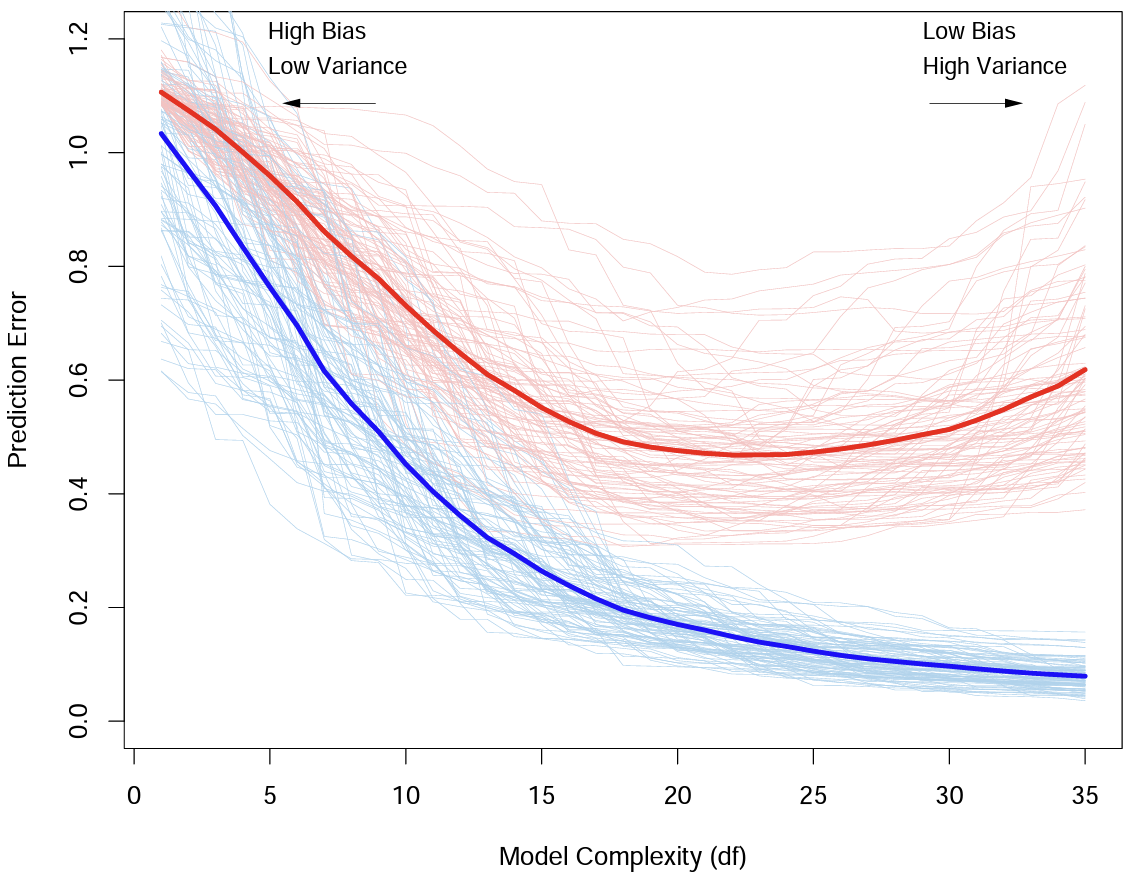
\includegraphics[scale=0.8]{images/model_selection_general_idea}
			\caption{Training (blue) vs text (red) error as the model complexity varies.}
		\end{figure}
	\end{frame}
	
	\begin{frame}
		\frametitle{Motivations - general idea}
		ML in one word: \textbf{generalization}!
		
		\vspace{5mm}
		
		Recall that we have to find a balance between fitting, on training data, and model complexity. Even though we limit the complexity of our model, training set does not provide a good estimate of test error.
		
		\vspace{5mm}
		
		In other words, generalization is compromised if we choose hyperparameters according to (only) training error.
	\end{frame}

	\begin{frame}
		\frametitle{Model selection and model assessment}
		Model selection: estimate the performance of different models trained with different hyperparameters. 
		
		\vspace{5mm}
		
		Model assessment: after choosing a final model we evaluate its perfomance on \textsl{completely new} test data.
		
		\vspace{5mm}
		
		N.B. Model selection and model assessment must be kept separated. Once we have chosen a final model, we are done with the model selection phase and model assessment is needed only to test the model on new data.
	\end{frame}

	\begin{frame}
		\frametitle{Double Hold out (Selection+Assessment)}
		\begin{figure}
			\centering
			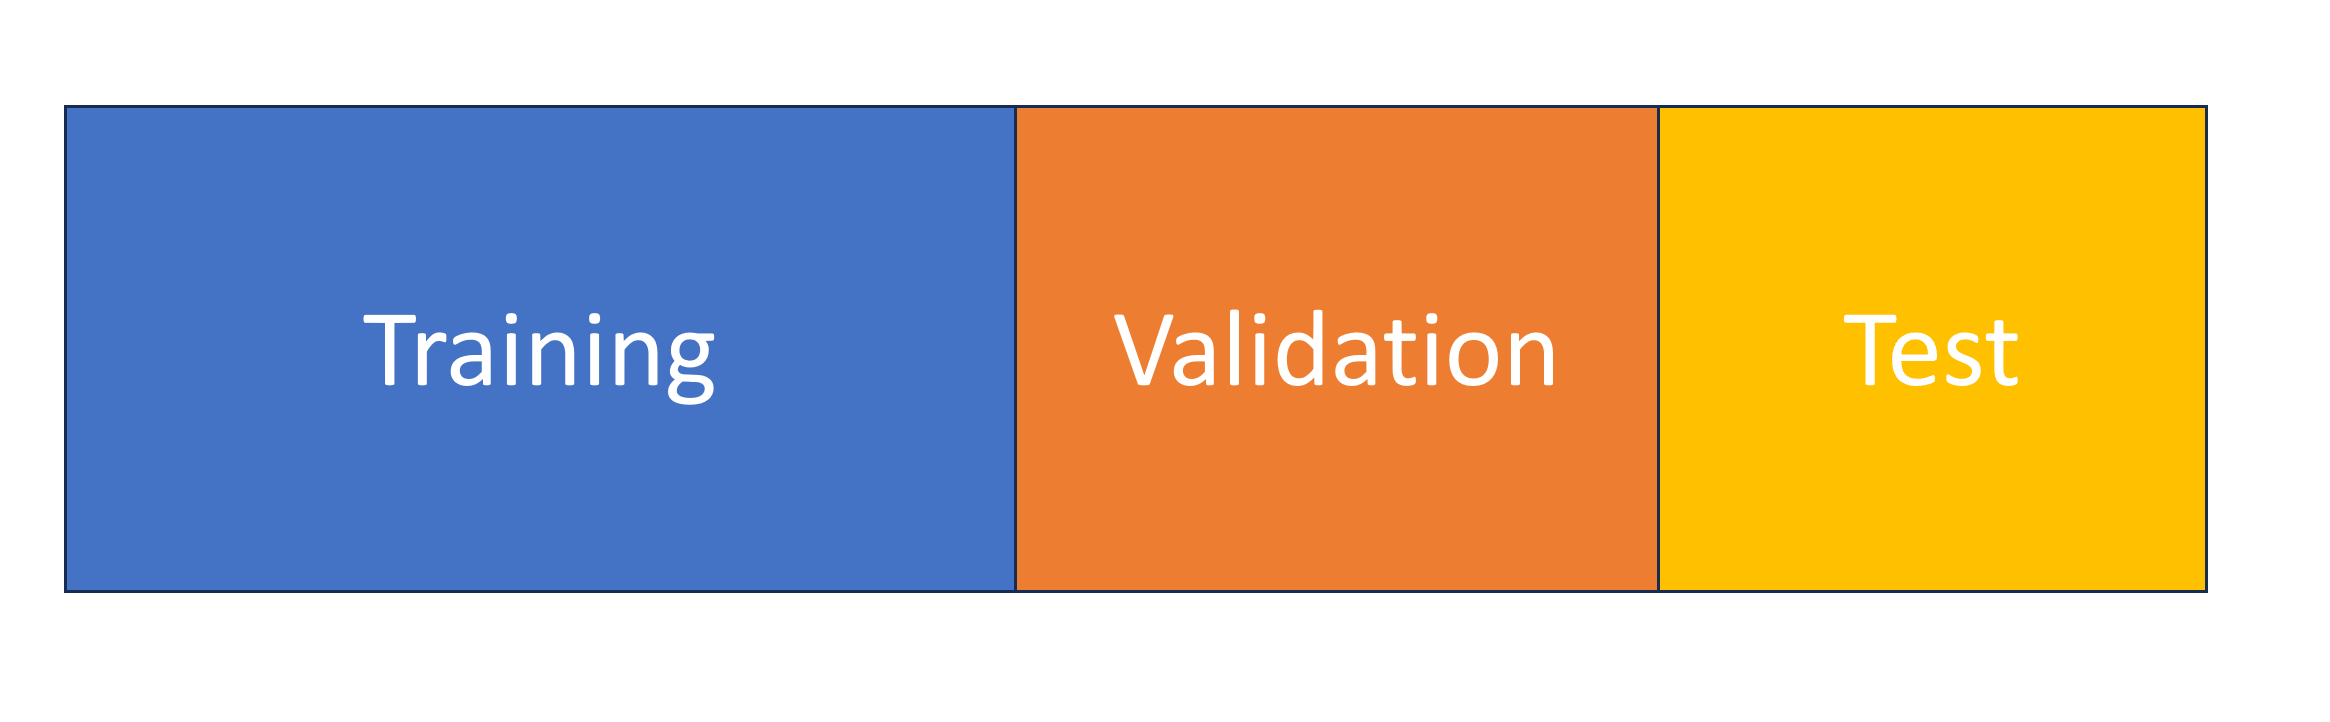
\includegraphics[scale=0.3]{images/hold-out}
		\end{figure}
		\begin{itemize}
			\item We split the entire dataset in three parts: training set, validation set and test set. Usually, training+validation constitutes the majority of the data available.
			\item Training set is used to fit. When the model is fitted, we evaluate its performance computing the error on the validation set.
			\textbf{Validation set is not a good estimation for the test error}.
			\item When a model is chosen, we evaluate its generalization capability computing the error on the test set. \textbf{Test set must not be used for hyperparameters selection}.
		\end{itemize}	
	\end{frame}

	\begin{frame}
		\frametitle{Cross validation (Selection or Assessment)}
		\begin{columns}
			\column{0.38\linewidth}
			\begin{figure}
				\centering
				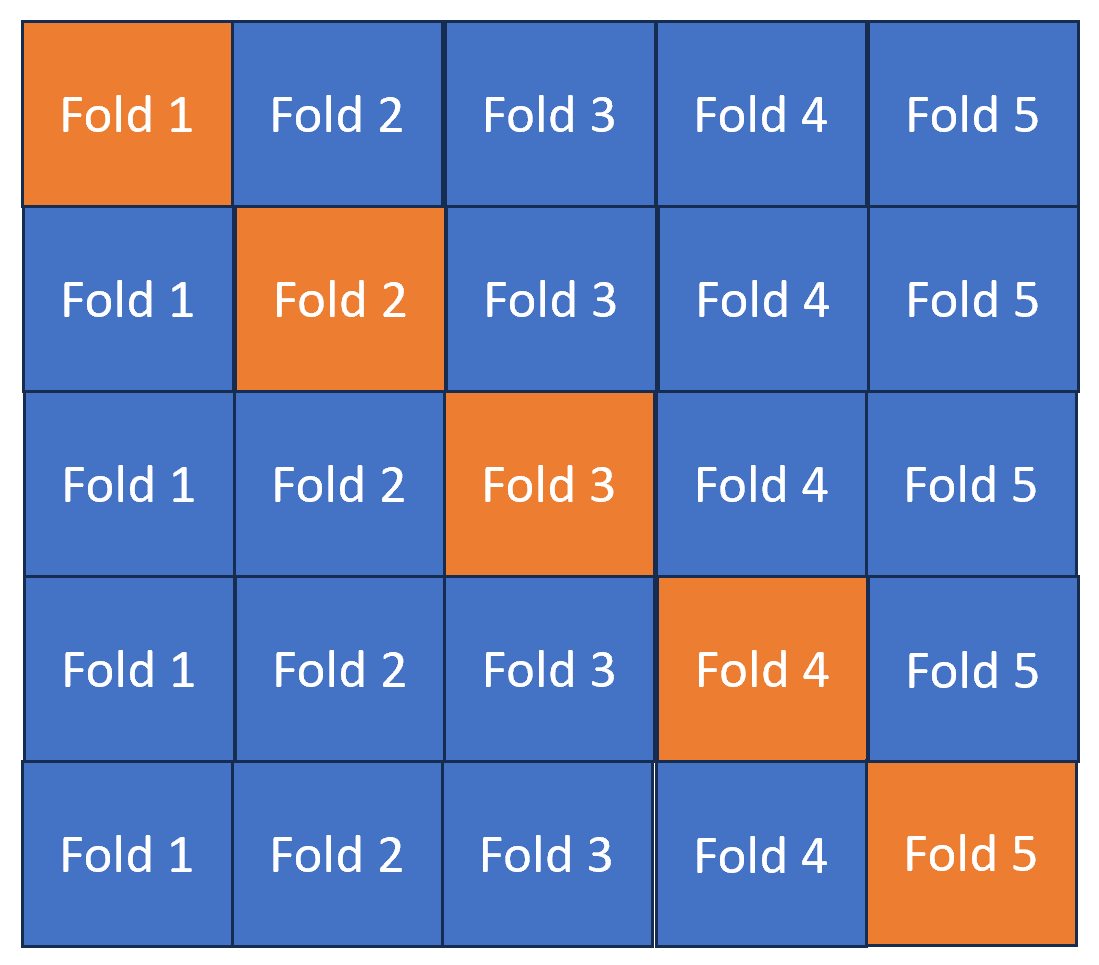
\includegraphics[scale=0.4]{images/cross-validation}
				\caption{5-fold CV}
			\end{figure}
			\column{0.58\linewidth}
			\begin{itemize}
				\item Split the data in $k$ disjoint folds.
				\item Use $k-1$ folds as the training set and the other fold as the validation set. Repeat it $k$ time (look figure).
				\item The performance will be the mean $\pm$ standard deviation computed across the $k$ runs.
			\end{itemize}
		\end{columns}
		Pro: Not sensible to a particular partition of the data. Mean filter the error.
		
		Contra: Computationally expensive (but parallellizable).
	\end{frame}

	\begin{frame}
		\frametitle{CV for selection and hold out for assessment}
		\begin{enumerate}
			\item Split dataset in two parts (hold out). One constitutes the development set $D$ (model selection), the latter is the test set $T$ (model assessment).
			\item Use the cross validation method on $D$ to select the best model.
			\item Evaluate its performance on the \textbf{external} test set $T$.
		\end{enumerate}
	
		Optional: after completing 2., hence after choosing the best hyperparameters and the best models, you can retrain (i.e. refit) the best model in the entire dataset $D$. In this way you exploit fully data you can for training.
	\end{frame}

	\begin{frame}
		\frametitle{Grid search (Selection)}
		
		How to search the best tuple of hyperparameters?
		
		\vspace{5mm}
		
		\textbf{Example}: two hyperparameters to choose (learning rate $\alpha$ and regularization parameter $\lambda$). Consider a set of values for both, e.g. $\alpha_{\text{vals}} = \{0.001, 0.01, 0.1\}, \lambda_{\text{vals}} = \{0.0001, 0.001, 0.01\}$. 
		
		Evaluate the model with $(\alpha, \lambda) = (i,j)$ for $i \in \alpha_{\text{vals}}, j \in \lambda_{\text{vals}}$.
		
		\begin{figure}
			\centering
			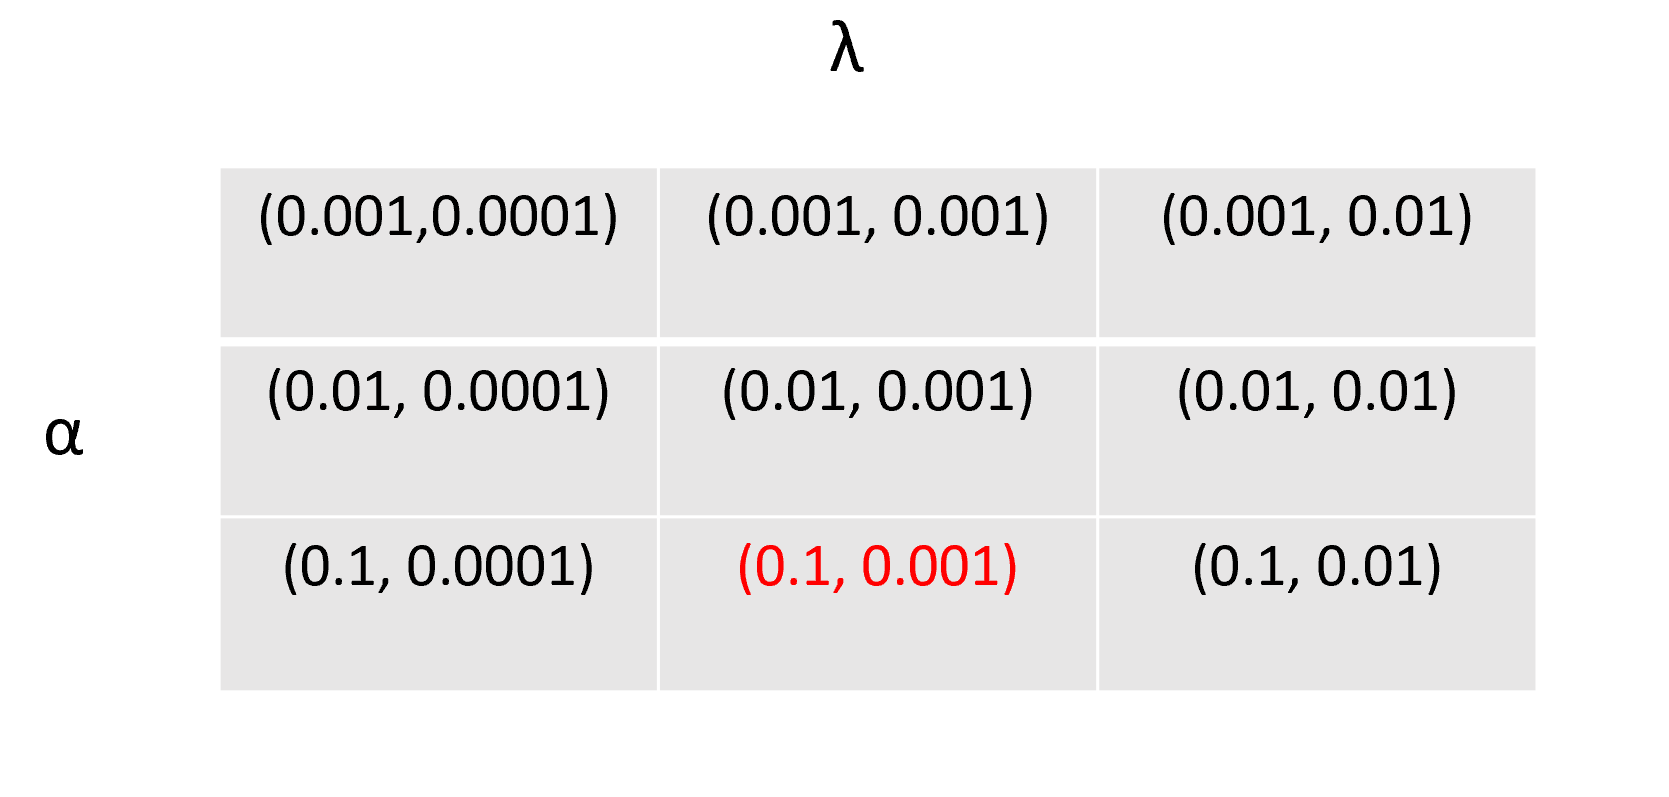
\includegraphics[scale=0.4]{images/grid-search}
		\end{figure}
		
		\textbf{Refinement}: Suppose that the best is $(0.1, 0.001)$. Then we can "zoom" near the best couple, doing another grid search with e.g. $\alpha_{\text{vals}} = \{0.075, 0.1, 0.125\}, \lambda_{\text{vals}} = \{0.00075, 0.001, 0.00125\}$. 
		
	\end{frame}

	\begin{frame}
		\frametitle{Bias and Variance definitions}
		\textbf{Bias}: discrepancy between true targets and the prediction of the current hypothesis.
		
		\vspace{5mm}
		
		\textbf{Variance}: variability of the predictions of the current hypothesis for different training data.
		
		\begin{figure}
			\centering
			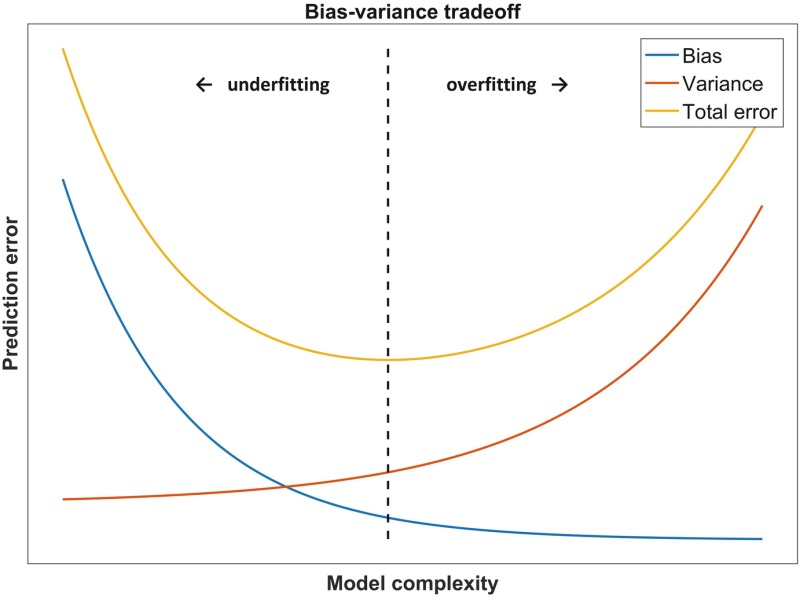
\includegraphics[scale=0.3]{images/bias-variance}
			\caption{Yellow curve: validation error.}
		\end{figure}
	\end{frame}

	\begin{frame}
		\frametitle{Bias-Variance: some intutitions}
		$\lambda$: regularization parameter.
		
		\vspace{5mm}
		
		\begin{itemize}
			\item High $\lambda$: high bias (underfitting).
			\item Low $\lambda$: high variance (overfitting)
			\item Intermediate $\lambda$: optimal solution.
		\end{itemize}
	
		\vspace{5mm}
		
		Complex model $\leadsto$ noise of the data captured $\leadsto$ high variance, low bias.
		
		\vspace{5mm}
		
		Simple model $\leadsto$ rigid hypothesis $\leadsto$ low variance, high bias.
	\end{frame}
\end{document}